\documentclass{standalone}

\usepackage{tikz}
\usetikzlibrary{chains}

\begin{document}
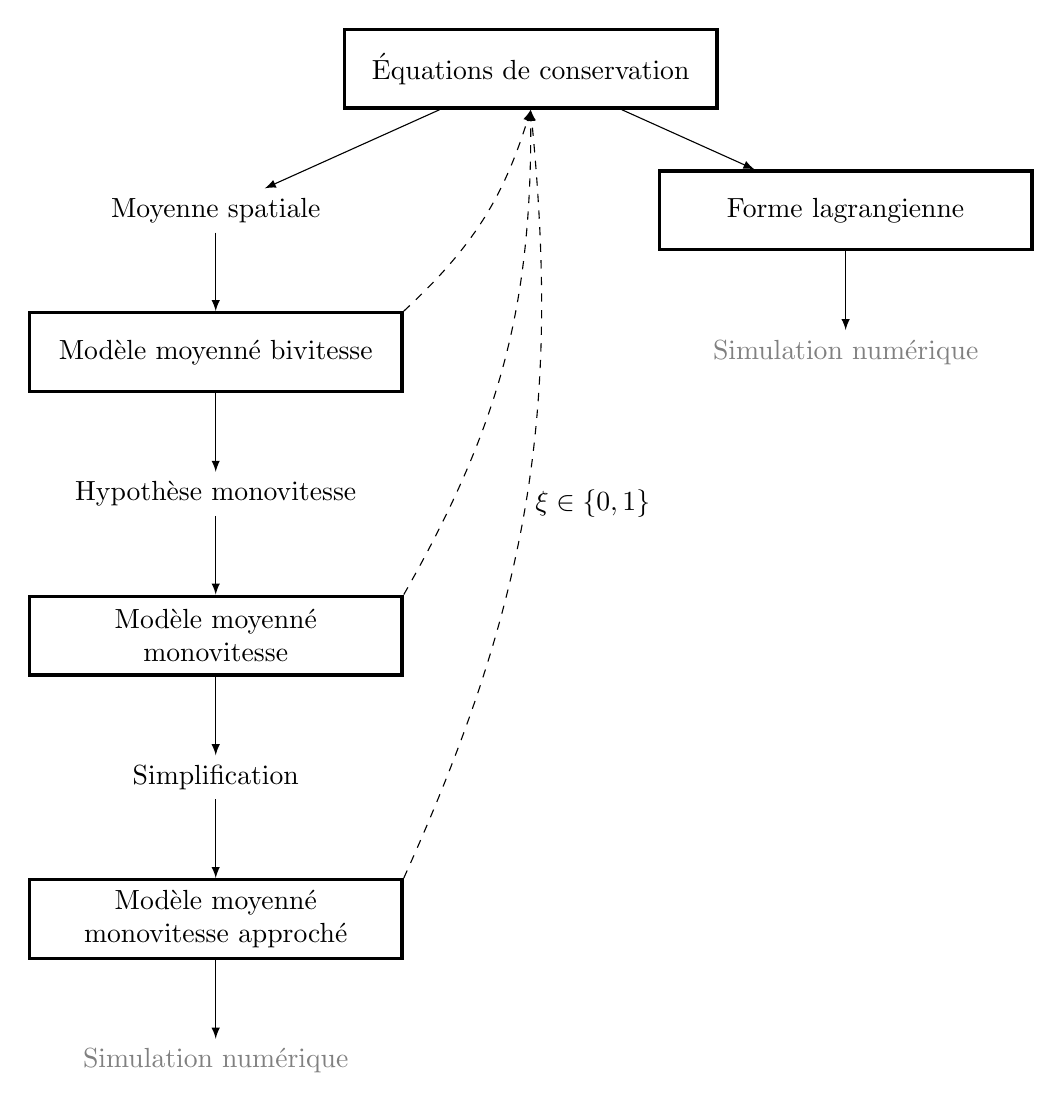
\begin{tikzpicture}
  [ start chain=going below,
    node distance=1.8cm and 4cm,
  every join/.style={dou}]		
  \tikzset{
    base/.style={
      on chain, on grid,
      align=center,
    },
    modele/.style={
      base,
      rectangle, 
      draw=black, very thick,
      minimum height=1cm, 
      text width=4.5cm, 
    },
    process/.style={
      base,
    },
    dou/.style={-latex, draw},
  }

  \node[modele, join] (modele) {Équations de conservation};

  \begin{scope}[start branch=euler]
    \node[process, on chain=going below left, join]      {Moyenne spatiale};
    \node[modele,  on chain=going below, join] (modmoy0) {Modèle moyenné bivitesse};
    \node[process, on chain=going below, join]           {Hypothèse monovitesse};
    \node[modele,  on chain=going below, join] (modmoy1) {Modèle moyenné\\monovitesse};
    \node[process, on chain=going below, join]           {Simplification};
    \node[modele,  on chain=going below, join] (modmoy2) {Modèle moyenné\\monovitesse approché};
    \node[process, on chain=going below, join, gray] (flux) {Simulation numérique};
  \end{scope}

  \begin{scope}[start branch=solveLagrange]
    \node[modele,  on chain=going below right, join]     {Forme lagrangienne};
    \node[process, on chain=going below, join, gray] (fluxic)  {Simulation numérique};
  \end{scope}

  \draw[-latex,  dashed] (modmoy2.north east) 
    to[bend right=15] 
    node[right] {$\xi \in \lbrace 0, 1 \rbrace$}
    (modele.south);
  \draw[-latex,  dashed] (modmoy1.north east) 
    to[bend right=15] 
    (modele.south);
  \draw[-latex,  dashed] (modmoy0.north east) 
    to[bend right=15] 
    (modele.south);
\end{tikzpicture}
\end{document}
